\documentclass[../main.tex]{subfiles}
\graphicspath{{\subfix{../images/}}}


\begin{document}
Python
\subsection{Libraries used}

Keras

Tensorflow (GPU)

Pandas

Numpy

Geopandas

Packages and programming language used.


\subsection{Data pre processing}

The years 2009 through 2018 is chosen to train and evaluate the model. All these files total approximately 130 gigabytes, which will introduce some limitation on how much of the data is processed at once. The process of finding possible routes in this raw data for further processing and validation involves finding all vessels that have visited the port of interest. Due to the file sizes and amount of data for each file this process has to be split into smaller chunks of time windows, \textit{i.e.} the number of consecutive months read in at once and processed. Due too the possibility of vessels starting a route at the end of a month but arriving the first day of the next month, larger time windows are preferred but limitations with memory limit this. Splitting the year into quarters proved to be a good compromise.

First step involves finding which vessels have visited the port of interest, the port of Naantali, for each month. This step is quite computationally time consuming, since every row in each file has to be checked, except rows of a previously known vessel. Only once a vessel has been identified to have visited the port of interest it can be skipped, else the row has to be checked. The process involves checking each rows latitude and longitude and whether the point is within the bounding box seen in Figure \ref{fig:FINLI-box}. This process has to be done once for each file, after which the unique identifiers for every vessel can be stored for future use. The raw files containing millions of row of data at average and begin around one gigabyte on file size limits the number of files that can be processed at once. Every month can have more than 30 unique vessels and the whole timeline has to extracted for all vessels.

\begin{figure}[H]
	\centering
	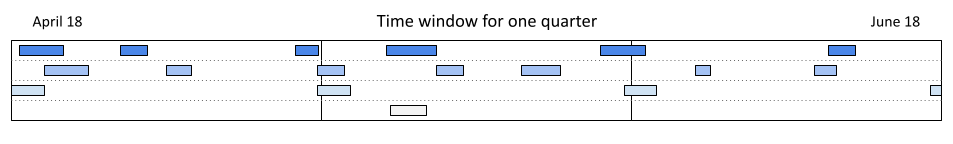
\includegraphics[scale=.45]{timeline.png}
	\caption{Example of one quarter of the the year 2018, a \textit{time window}, and from this time window each unique vessels complete timeline is extracted for further processing. The coloured boxes represents raw AIS data for four unique vessels. Does not represent actual data, rather visualizing the process of finding relevant data in the raw HELCOM dataset.}
	\label{fig:timeline}
\end{figure}

From the complete time window seen in Figure \ref{fig:timeline} only a fraction is used for the final route finding algorithm, see Table \ref{tab:HELCOM-data-percent}. Joining this raw AIS data for every vessel found generates a timeline for each vessel.

\subsubsection{Algorithm for extracting routes from dataset}

Explain the algorithm behind getting the routes from the raw data set and that the idea can be applied to any port or area of interest really by defining the area of interest.

\begin{algorithm}[H]
\SetAlgoNoLine
\SetAlgoNoEnd

\SetKwData{Index}{index}\SetKwData{End}{end}\SetKwData{Start}{start}
\SetKwData{Route}{route}\SetKwArray{R}{R}
\KwIn{DataFrame for one vessel sorted in descending time, a \textit{timeline}}
\KwResult{List \R of all routes found}
\emph{The algorithm searches in reverse order of time from reaching the destination until the start of the route}\;
\BlankLine
\ForEach{row in DataFrame}{
	\Index $\leftarrow$ Keep track of current row\;
	\BlankLine
	\If(\tcp*[f]Only true after finding first route){\Route found}{
		\emph{Start searching from first unknown point}\;
		Skip rows until \Index $=$ \Start\;
	}
	\BlankLine
	\If{current point is in PORT}{
		\ForEach{row in DataFrame starting from \Index}{
			\If(\tcp*[f]Vessel is entering the port){point is outside PORT}{
				\End $\leftarrow$ First point reaching the destination\;
				\BlankLine
				\ForEach{row in DataFrame starting from \End}{
					
					\If{start of route reached}{
						\Start $\leftarrow$ Current row\;
						\R $\leftarrow$ Save route from \End to \Start\;
					}
				}
			}
		}
		\tcc{When a route has been found and saved start search again from the last not visited point.}
	}
}
\caption{Find all routes going to a area of interest}
\label{alg:search}
\end{algorithm}
\vspace*{5mm}
The end of a route is either vessels sog less than 0.1 for more than 5 consecutive messages or has travelled longer than 48 hours

Duration of route travel time 

Minimum distance travelled

The largest gaps allowed 12 minutes

Travelling back to FINLI

Faulty data that can not be inferred from other data example draught

The port chosen for the evaluation has its caveats and should perhaps be identified.

Validation of the routes extracted i.e gaps, no shorter than n number of messages where the vessel is going, not returning to port, longer than n hours, no faulty data etc.

\begin{figure}[H]
	\centering
	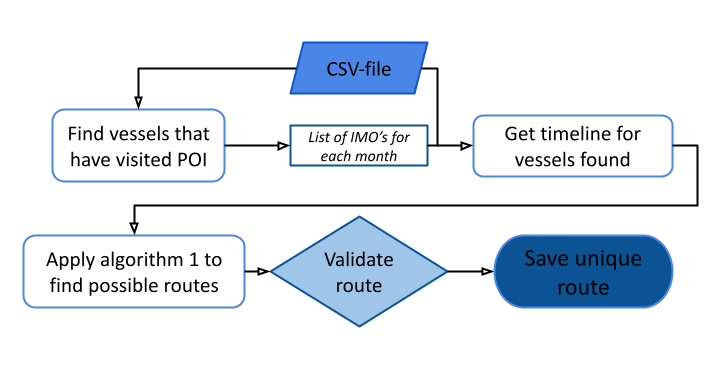
\includegraphics[scale=.5]{data-process.png}
	\caption{Getting routes.}
	\label{fig:flowchart}
\end{figure}

\begin{figure}[H]
	\centering
	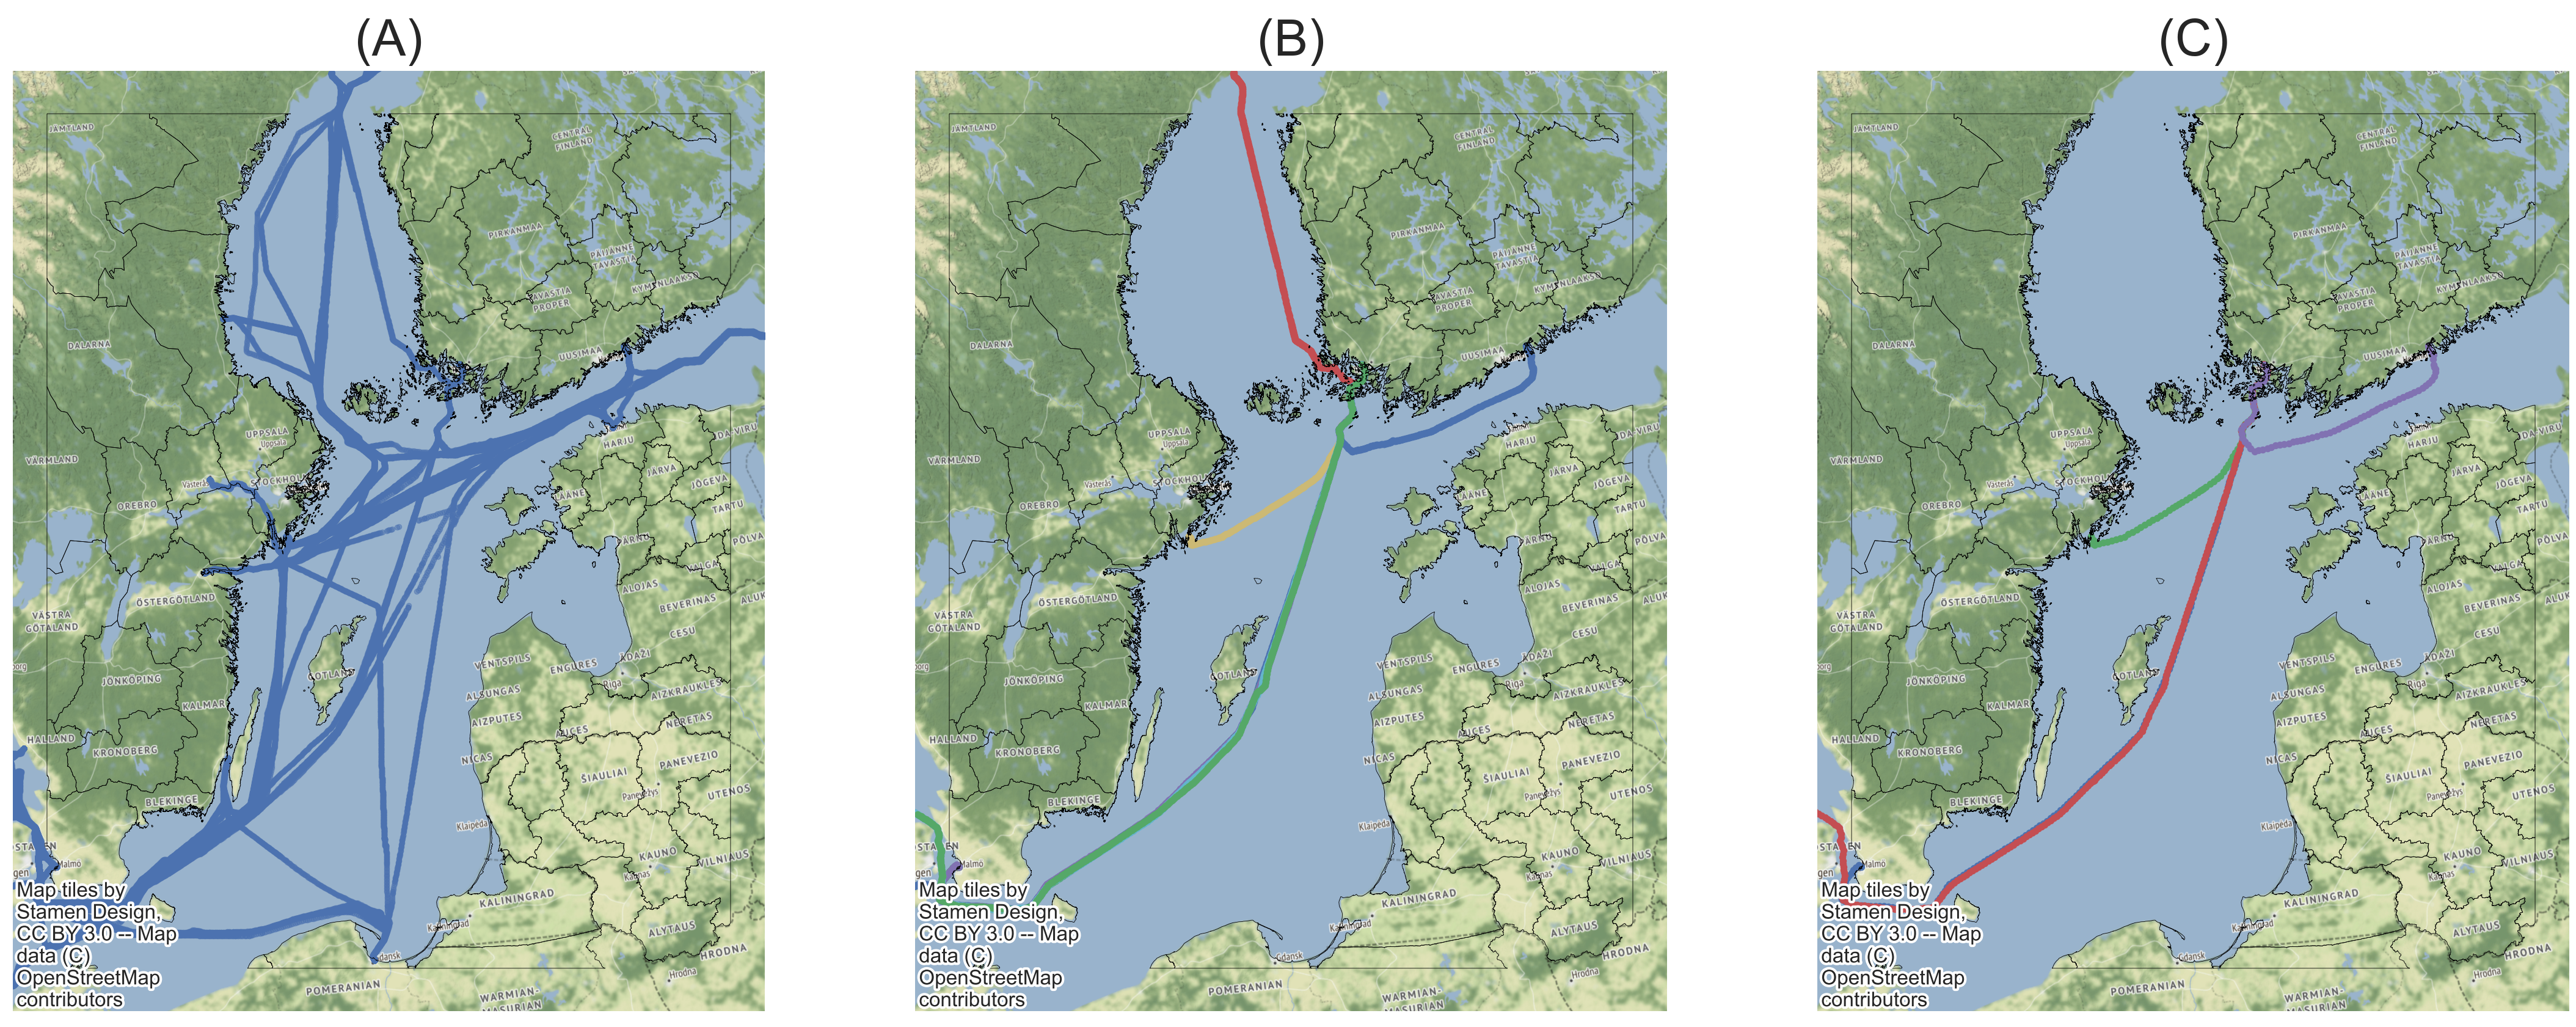
\includegraphics[scale=.45]{route-finding-9256420.png}
	\caption{(A) Complete timeline for one vessel year 2013. (B) All possible routes for the same vessel. (C) All validated routes which are used for training. }
	\label{fig:route-finding}
\end{figure}

The number of routes found from each complete year was at average 1395 routes. 

The total number of routes for the period chosen was 13,955. However, only a fraction of these routes are valid routes. The final route validation and which rules are defined to find viable routes are explained in the next section.
What range of data was used for the final model and reason for so. The problems with AIS data and getting clean routes from start to finish and primarily enough routes for training and testing. 

POI (port of interest could also be thought of as Area of Interest). Timeline is the vessels historical data which is fed into algorithm 1. Route validation according to rules and then save the complete route.

\subsubsection{Coordinate accuracy}

The latitude and longitude recorded in the HELCOM dataset with an accuracy of six decimal places, 0.111 meters, is not necessary.

The level of scaling the coordinate accuracy was chosen to a decimal degree of three places. That will say 0.001 which is 111 meters. The accuracy of the vessels location will be within approximately 100 meters.

\begin{table}[H]
\centering
\begin{tabular}{|l|c|}
\hline
\rowcolor[HTML]{9B9B9B} 
\textbf{Degrees} & \multicolumn{1}{l|}{\cellcolor[HTML]{9B9B9B}\textbf{Distance}} \\ \hline
1.0              & 111 km                                                         \\ \hline
\rowcolor[HTML]{EFEFEF} 
0.1              & 11.1 km                                                        \\ \hline
0.01             & 1.11 km                                                        \\ \hline
\rowcolor[HTML]{EFEFEF} 
0.001            & 111 m                                                          \\ \hline
0.0001           & 11.1 m                                                         \\ \hline
\rowcolor[HTML]{EFEFEF} 
0.00001          & 1.11 m                                                         \\ \hline
\end{tabular}
\caption{Coordinate accuracy by decimal places in decimal degrees for latitude and longitude, from \textbf{ref GIS wiki}}
\label{tab:gis-accuracy}
\end{table}

AIS messages transmitted within approximately 100 meters of each other will be thought of as sent from the same location using this scaling level.

Vessel travelling at 14 knots (25 km/h) and a message interval of 10 minutes approx. will move 2.2 nmi (4.1 km) per message



\subsubsection{Feature selection}

The features chosen for the final training 

Latitude, longitude, sog, cog, vessel class, draught, ?distance? 

The target is Time To Destination, how many minutes are left to the destination


\subsubsection{Time series data preparation and cleanliness}

Further details on how the processed routes are handled to generate the training data to utilize multiple timesteps per prediction which improves performance. Also why the number of timesteps per prediction was chosen, with the time normalized data and how many steps then per time window. 

The largest allowed difference between messages in the time normalized data

\subsection{ML model}

Description of the neural network model used and tested to find the optimal performer


\subsection{Comparison model}

!!! If the travel distance left to destination is used in nmi for example, test the accuracy against simply calculating time left by the current speed and distance left 

\end{document}